\documentclass[dvipsnames,pdflatex,beamer]{beamer}
\usepackage[english]{babel}
\usepackage[utf8]{inputenc}
%beamer breaks with\usepackage{paralist}%-> {compactenum}, ... (Aargh!)
%\usepackage{mdwlist}% \suspend and \resume enumerate
\usepackage{relsize}% ``relative font sizes''
%% part of {mmVignette} below: \usepackage{SweaveSlides}
\usepackage{mmVignette}%-- local in this directory: -> {listings}, \lstset,...
%           ^^^^^^^^^^
\usepackage{MM-slides}% whitespace-tricks, \nlQ etc
\usepackage{MM-colors}% {\color{salmonII} ..text..} \textcolor{red}{..txt..}
%\usepackage{bm}
%-------------------------------------------------------------
%
\newcounter{saveenum}
\newcommand{\Rp}{\textsf{R}}
\renewcommand{\R}{\Rp\ }
%fails: why? \def\Rp\RR% and \RR is in mmVignette -- R program
\newcommand*{\CRAN}{\textsc{cran}$\;$}
\newcommand*{\W}{\ensuremath{\mathbf{W}}}
\newcommand*{\Ip}{\mathbf{I}_p}
%---- from texab.sty --- can not take all --------------
% \newcommand{\norm}[1]   {\left\| #1 \right\|}
% % the above sometimes give much too long  || -- then use the following:
% \newcommand{\normb}[1]  {\bigl\|{#1}\bigr\|}
% \newcommand{\normB}[1]  {\Bigl\|{#1}\Bigr\|}
\newcommand{\fn}[1]{\kern-2pt\left(#1\right)}
\newcommand{\Ew}[1]{\mathbf{E}\kern2pt\fn{#1}}
\DeclareMathOperator{\logit}{logit}
%
%
\mode<handout>{\usetheme{default}}
\mode<beamer>{%
  %%> http://www.namsu.de/latex/themes/uebersicht_beamer.html
  \usetheme{Boadilla}% somewhat similar to Singapore, but "nice" blocks
  %\usetheme{Singapore}%  \usetheme{Madrid}%
  \setbeamercovered{dynamic}% {transparent} {invisible} or {dynamic}
  % Use ETH Logo
%   \pgfdeclareimage[height=0.5cm]{ETH-logo}{../ethlogo_black}%
%   \logo{\pgfuseimage{ETH-logo}}%
  % \pgfdeclareimage[height=0.5cm]{R-logo}{Rlogo}%
  \pgfdeclareimage[height=0.5cm]{R-logo}{useR}%
  \logo{\pgfuseimage{R-logo}}%
}
\usefonttheme[onlymath]{serif}


\title[Arbitrarily Accurate R: Package 'Rmpfr']{%
  Arbitrarily Accurate Computation with R: \\ The 'Rmpfr' Package}

\author[Martin M\"achler]{Martin M\"achler}
\institute[R Core/ ETH Zurich]{% 'ETH Z' if more needed
  \begin{minipage}{.44\textwidth}
  \begin{flushleft}
  {\color{Scode}\texttt{maechler@R-project.org} \ \  \ \ (R-Core)}\\
  {\color{Scode}\texttt{maechler@stat.math.ethz.ch}  \ (ETH)}
\end{flushleft}
\end{minipage}

  \bigskip

  Seminar für Statistik \\ ETH Zurich  \ \ Switzerland
}
%\date[useR! @ Warwick, 2011]{useR! 2011, Warwick \\ August 16, 2010}
\date[ZurichR @ ETH, Jan.2012]{ZurichR @ ETH, Jan.19, 2012}
\AtBeginSection[]%-- at the beginning of every new section, do the following
{
  \begin{frame}<beamer>
    \frametitle{Outline}
    \tableofcontents[currentsection,hideallsubsections]
  \end{frame}
}
\begin{document}

\begin{frame} \titlepage
\end{frame}
%
\begin{frame} \frametitle{Outline}
  \tableofcontents[hideallsubsections]
  % You might wish to add the option [pausesections]:
  %\tableofcontents[pausesections,hideallsubsections]
\end{frame}

\section{Example: 16 digits are not always enough!}\label{sec:intro}


\setkeys{Gin}{width=\textwidth}

\subsection{Simple (semi-artificial!) Example: logit(exp(-L))}
\begin{frame}[fragile]
  Logistic regression: Computing ``logit()''s, $\log \frac{p}{1-p}$
  accurately for very small $p$, i.e., $p = \exp(-L)$, or
  \vspace*{-.6ex}
  \[
  \log\frac{p}{1-p} = \log p - \log(1 - p) = -L - \log(1 - \exp(-L)),
  \]
  \vspace*{-.5ex}

  and hence $-\log(1 - \exp(-L))$ is needed, e.g.,
  when p is really really close to 0, say $p = 10^{-1000}$, as then
  we can only compute $\logit(p)$, if we specify  $L := -\log(p) \leftrightarrow p = \exp(-L)$.

\begin{Schunk}
\begin{Sinput}
> curve(-log(1 - exp(-x)), 0, 10)
\end{Sinput}
\end{Schunk}
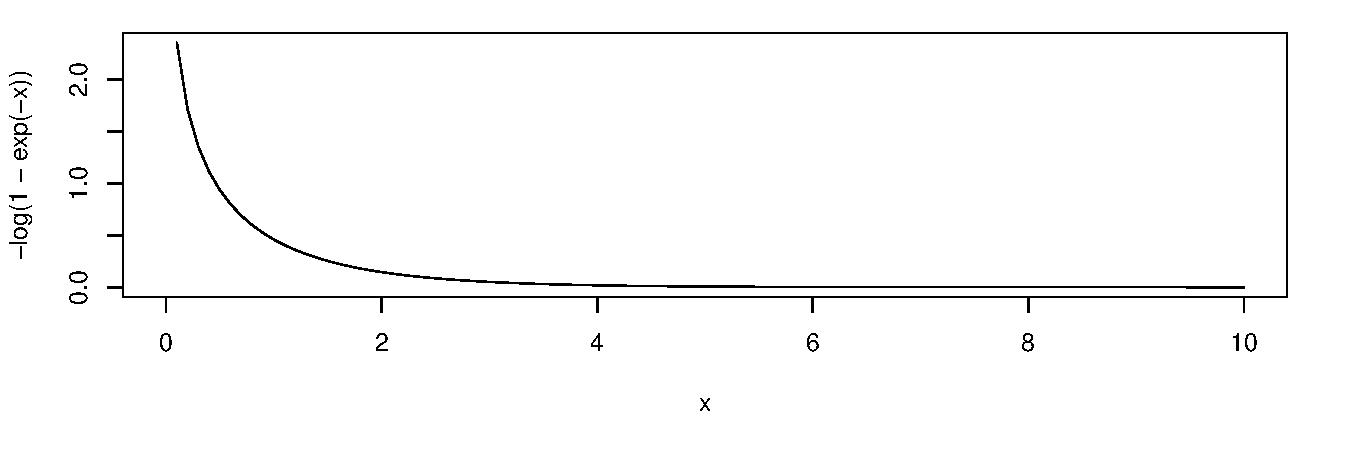
\includegraphics{log1exp-log1-exp-curve-10}

seems fine. --- ---  However, \dots
\end{frame}

\begin{frame}[fragile]
However, further out to 50 (and on a log scale), we observe

\begin{Schunk}
\begin{Sinput}
> curve(-log(1 - exp(-x)),  0, 50, log="y")
\end{Sinput}
\end{Schunk}
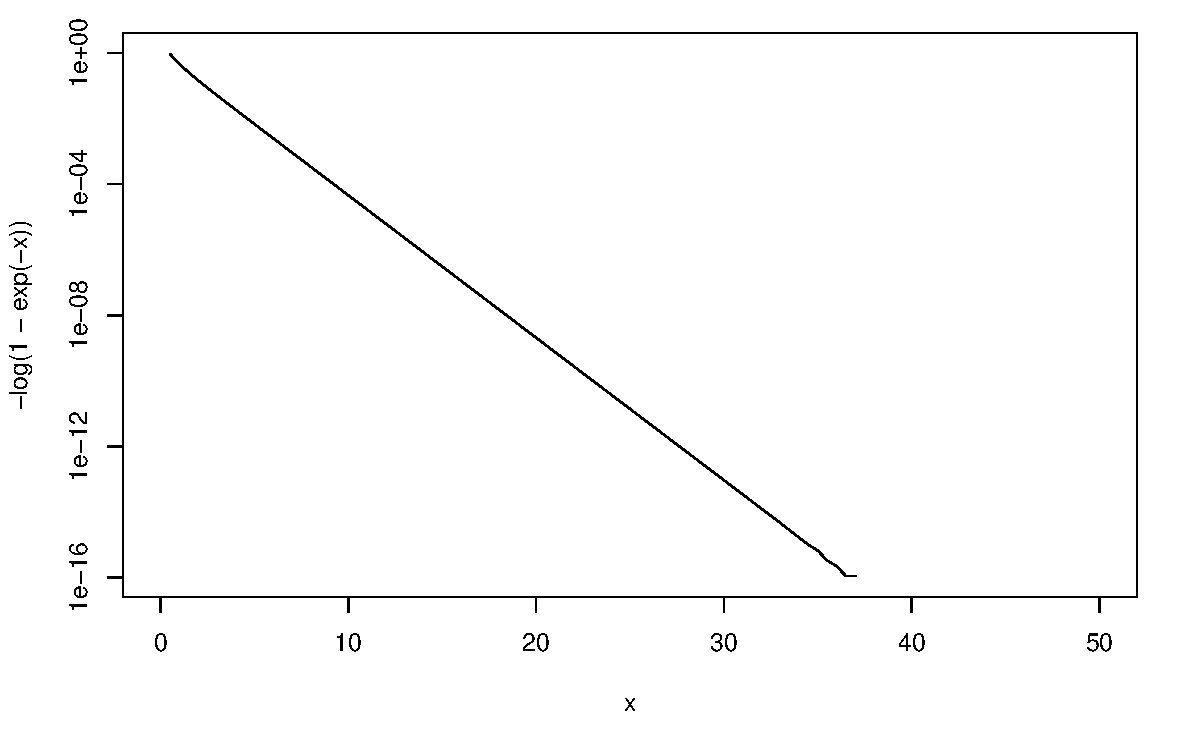
\includegraphics{log1exp-log1-exp-curve-log}
\\[-.6ex]
which shows early underflow.
\end{frame}

\begin{frame}[fragile]
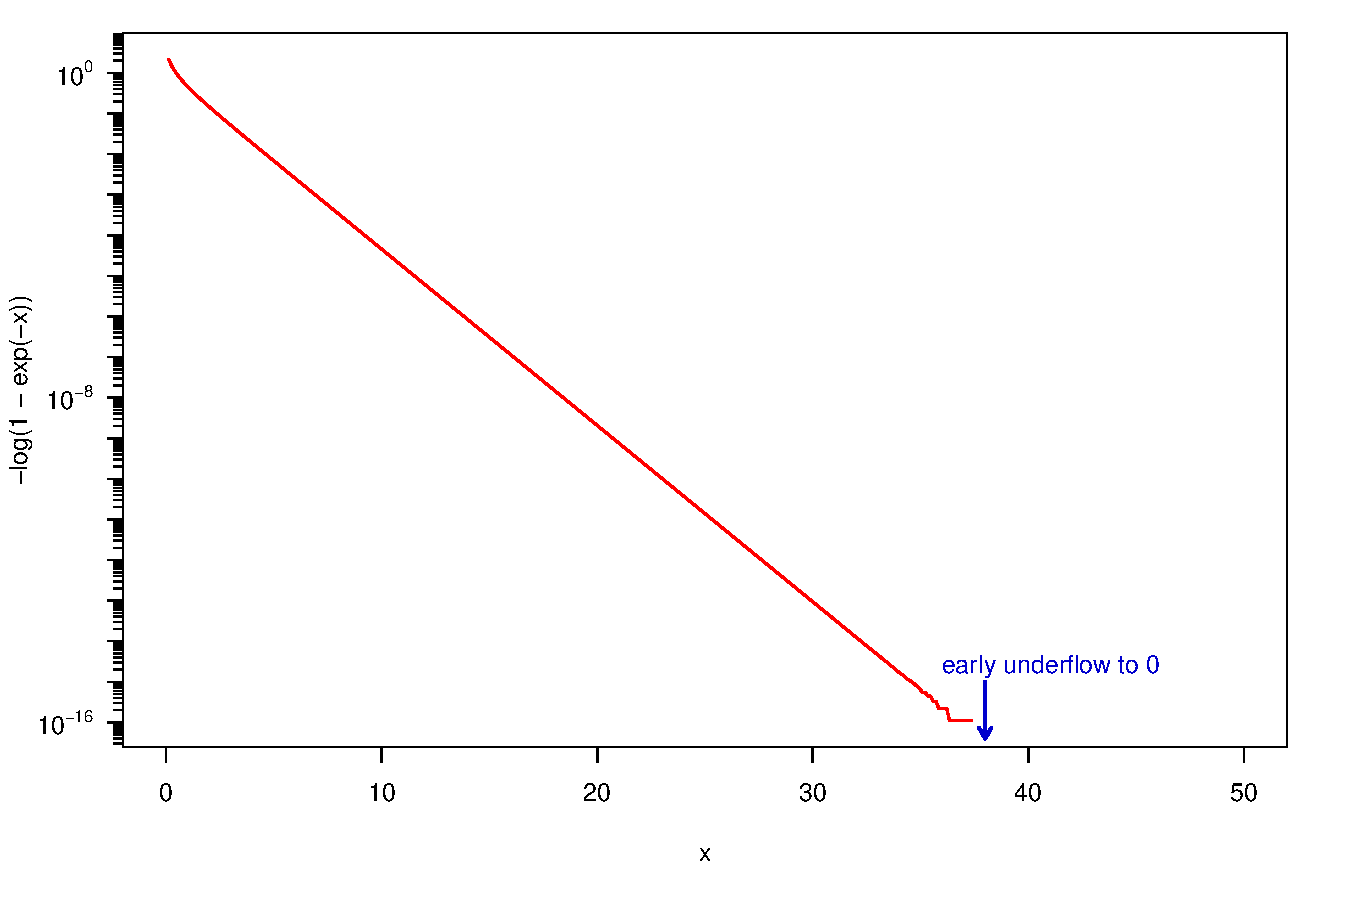
\includegraphics{log1exp-log1-exp-log-niceer}
\end{frame}

\begin{frame}[fragile]
What did happen?  Look at
\begin{Schunk}
\begin{Sinput}
> x <- -40:-35
>     -log(1 - exp(x))
\end{Sinput}
\begin{Soutput}
[1] 0.000000e+00 0.000000e+00 0.000000e+00 1.110223e-16 2.220446e-16
[6] 6.661338e-16
\end{Soutput}
\begin{Sinput}
> log(-log(1 - exp(x)))# --> -Inf values
\end{Sinput}
\begin{Soutput}
[1]      -Inf      -Inf      -Inf -36.73680 -36.04365 -34.94504
\end{Soutput}
\begin{Sinput}
> ## ok, how about more accuracy
> x. <- mpfr(x, 120)
> log(-log(1 - exp(x.)))# aha... looks perfect now
\end{Sinput}
\begin{Soutput}
6 'mpfr' numbers of precision  120   bits 
[1] -39.999999999999999997932904877538241734
[2]  -38.99999999999999999423372196756935807
[3]  -37.99999999999999998430451715981029611
[4] -36.999999999999999957331848579613165434
[5] -35.999999999999999884024061830552087239
[6] -34.999999999999999684744214015307532692
\end{Soutput}
\end{Schunk}
\end{frame}

\begin{frame}[fragile]
And visually:
\begin{Schunk}
\begin{Sinput}
> x <- seq(-40, -20, by = .5)
> plot(x,x, type="n", ylab="", ann=FALSE)
> lines(x, log(-log(1 - exp(x))), type = "o", col = "purple", lwd=3, cex = .6)
\end{Sinput}
\end{Schunk}
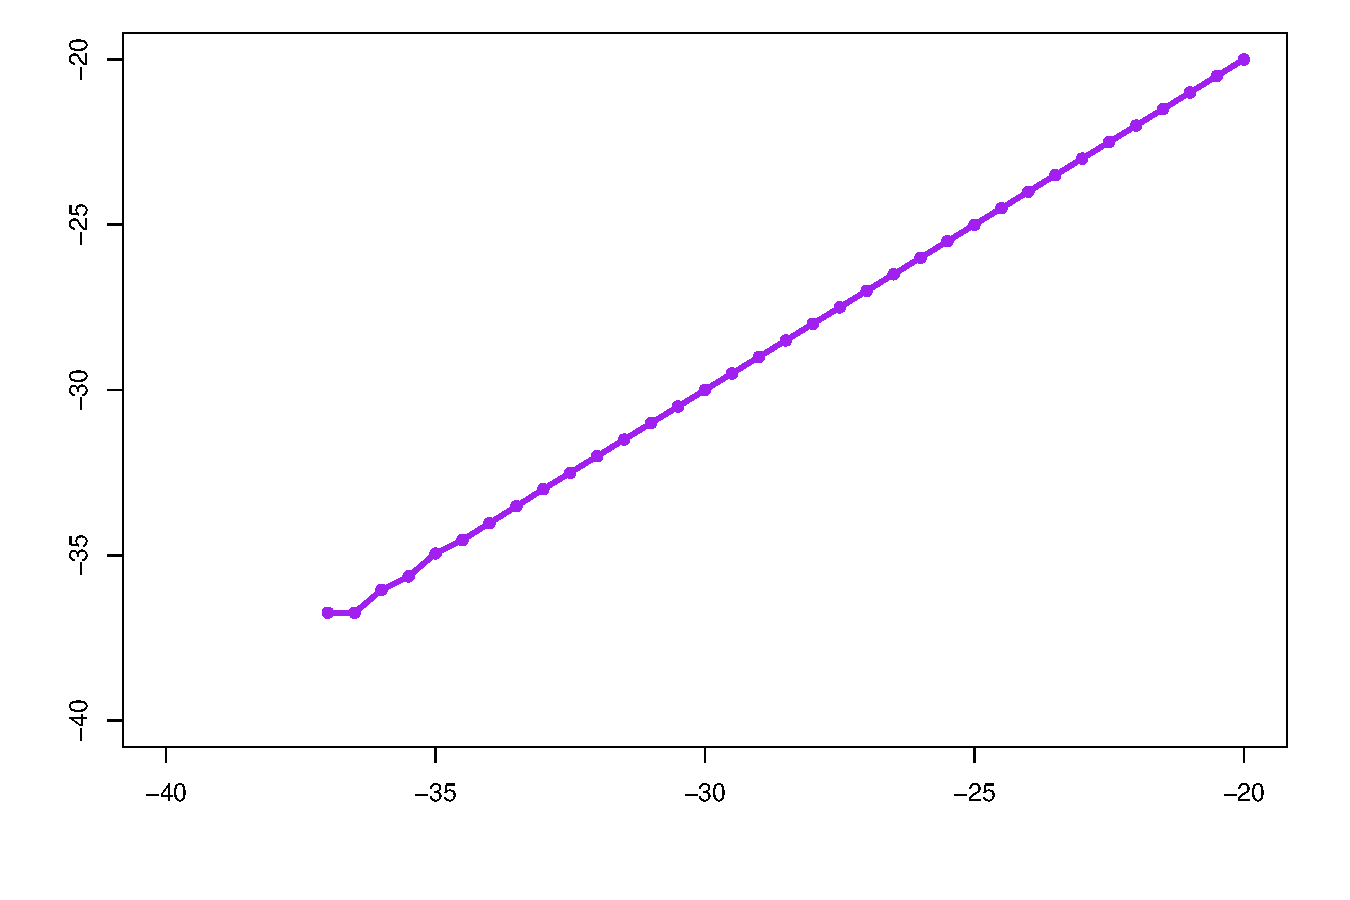
\includegraphics{log1exp-plot-log1exp-ex}
\end{frame}

\begin{frame}[fragile]
Now repeat this with ``with accuracy'':
\begin{Schunk}
\begin{Sinput}
> x <- seq(-40, -20, by = .5)
> plot(x,x, type="n", ylab="", ann=FALSE)
> lines(x, log(-log(1 - exp(x))), type = "o", col = "purple", lwd=3, cex = .6)
> x. <- mpfr(x, 120)
> lines(x, log(-log(1 - exp(x.))), col=2, lwd=1.5)
\end{Sinput}
\end{Schunk}
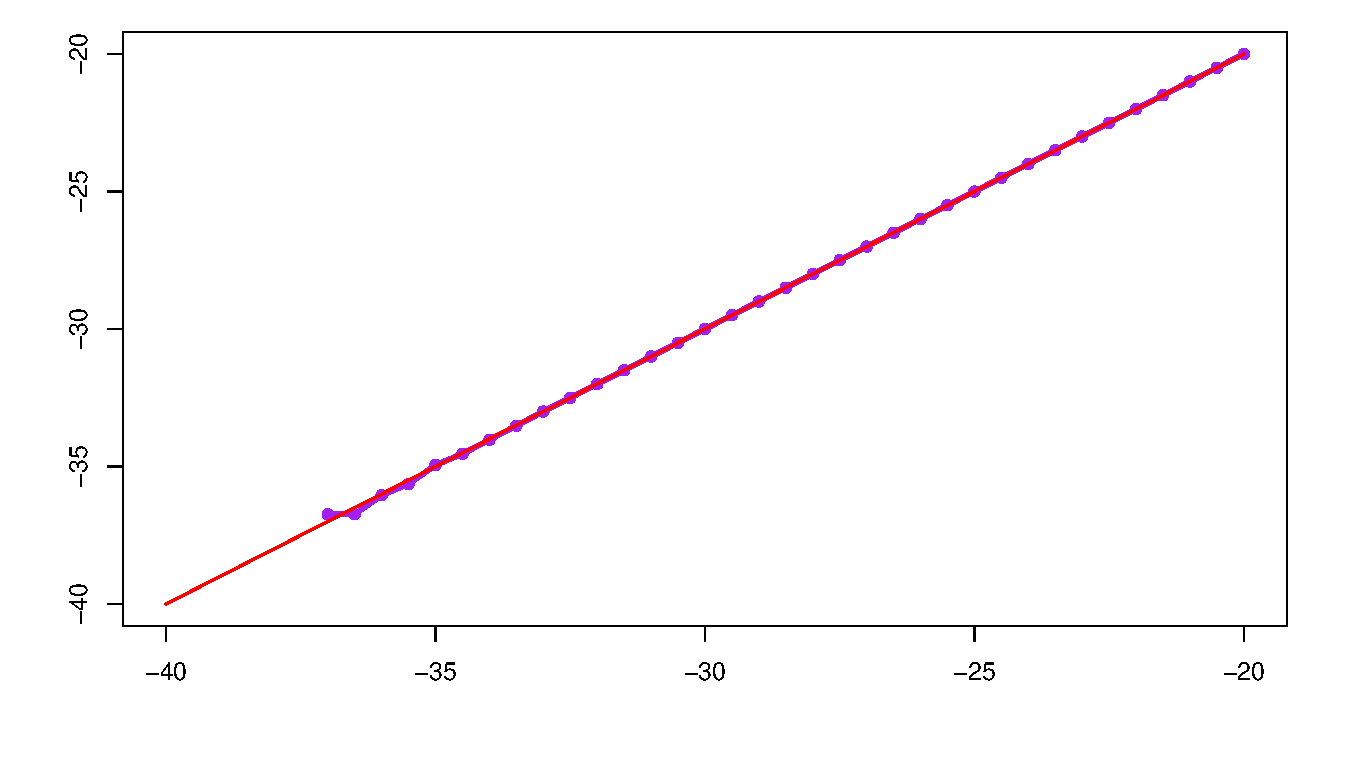
\includegraphics{log1exp-plot-log1exp-mpfr}
\end{frame}


%%% Local Variables:
%%% TeX-command-default: "LaTeX PDF"
%%% TeX-master: "Maechler_Rmpfr.tex"
%%% End:


%%     =======
\section{Example 2: Exact Factorials and Binomial Coefficients}\label{sec:BinCoef}


\setkeys{Gin}{width=\textwidth}

\subsection{Exact Factorials and Binomial Coefficients}
%% From ~/R/Pkgs/Rmpfr/inst/doc/Rmpfr-pkg.tex
%% ---------------------------------------
\begin{frame}[fragile]\frametitle{Exact Factorials and Binomial Coefficients}
In combinatorics or when computing series,
work with \emph{exact} factorials or binomial coefficients.
E.g.,need all factorials $k!$, for $k=1,2,\dots,24$ or a full row
of Pascal's triangle, i.e., want all $\binom{n}{k}$ for $n=50$.

With \Rp's double precision,
% and standard printing precision
% <<factorial-1>>=
% ns <- 1:24 ; factorial(ns)
% @
% the full precision of $24!$ is clearly not printed. However,
and if you display its full internal precision,
\begin{Schunk}
\begin{Sinput}
> noquote(sprintf("%-30.0f", factorial(24)))
\end{Sinput}
\begin{Soutput}
[1] 620448401733239409999872      
\end{Soutput}
\end{Schunk}
\smallskip
then it is obviously wrong for $24!$, as its last digits are known to be \code{0}.

\medskip

Easily get full precision results, by
replacing ``simple'' numbers by ``mpfr''s:
\begin{Schunk}
\begin{Sinput}
> ns <- mpfr(5:24, 120) ; factorial(ns)
\end{Sinput}
\end{Schunk}
\begin{Schunk}
\begin{Soutput}
20 'mpfr' numbers of precision  120   bits 
 [1]                      120                      720
 [3]                     5040                    40320
 [5]                   362880                  3628800
 [7]                 39916800                479001600
 ....... 
 ....... 
[13]          355687428096000         6402373705728000
[15]       121645100408832000      2432902008176640000
[17]     51090942171709440000   1124000727777607680000
[19]  25852016738884976640000 620448401733239439360000
\end{Soutput}
\end{Schunk}
\end{frame}

\begin{frame}[fragile]
Or for the 70-th Pascal triangle row, $\binom{n}{k}$ for $n=70$ and $k=0,\dots,n$,
\begin{Schunk}
\begin{Sinput}
> chooseMpfr.all(n = 70)
\end{Sinput}
\end{Schunk}
\begin{Schunk}
\begin{Soutput}
70 'mpfr' numbers of precision  67   bits 
 [1]                    70                  2415                 54740
 [4]                916895              12103014             131115985
 [7]            1198774720            9440350920           65033528560
[10]          396704524216         2163842859360        10638894058520
 ....... 
 ....... 
[25]   6455761770304780752  11173433833219812840  18208558839321176480
[28]  27963143931814663880  40498346384007444240  55347740058143507128
[31]  71416438784701299520  87038784768854708790 100226479430802391940
[34] 109069992321755544170 112186277816662845432 109069992321755544170
 ....... 
 ....... 
[67]                 54740                  2415                    70
[70]                     1
\end{Soutput}
\end{Schunk}
\end{frame}

%%% TeX-master: "Maechler_Rmpfr.tex"

%%     =======
\section{Alternating Binomial Sums}


\setkeys{Gin}{width=\textwidth}

%\subsection{Alternating Binomial Sums}
%% From ~/R/Pkgs/Rmpfr/inst/doc/Rmpfr-pkg.tex
%% or rather, the result of
%%    R CMD Rdconv --type=latex ~/R/Pkgs/Rmpfr/man/sumBinomMpfr.Rd
%%                            ---------------------------------------

\begin{frame}\frametitle{Alternating Binomial Sums}
Alternating binomial sums
appear in different contexts and are typically challenging,
i.e., currently impossible, to evaluate reliably as soon as $n$ is
larger than around $50 - 70$.

The alternating binomial sum $sB(f,n) :=$ \texttt{sumBinom(n, f, n0=0)} is
(up to sign) equal to the $n$-th forward difference operator $\Delta^n f$,
\begin{equation} \label{eq:sumBin}
 sB(f,n) := \sum_{k=0}^{n} (-1)^k {n \choose k}\cdot f(k) = (-1)^n \Delta^n f,
\end{equation}
where
\begin{equation}
  \label{eq:sumBin2}
  \Delta^n f = \sum_{k=0}^{n} (-1)^{n-k}{n \choose k}\cdot f(k)
\end{equation}
is the $n$-fold iterated forward difference
$\Delta f(x) = f(x+1) - f(x)$  (for $x = 0$).
\end{frame}

\begin{frame}[fragile]\frametitle{computing alternating binomial sums in R}
An obvious R implementation of
\(
 sB(f,n) = \sum_{k=0}^{n} (-1)^k {n \choose k}\cdot f(k)
\),
\medskip

\begin{Schunk}
\begin{Sinput}
> sumBinom <- function(n, f, n0=0, ...) {
+   k <- n0:n
+   sum( choose(n, k) * (-1)^k * f(k, ...))
+ }
> ## and the same for a whole *SET* of  n  values:
> sumBin.all.R <- function(n, f, n0=0, ...)
+    sapply(n, sumBinom, f=f, n0=n0, ...)
\end{Sinput}
\end{Schunk}
\bigskip

Will see: gets numerical problems, for relatively small $n$ even for well
behaved functions $f(\cdot)$.
\end{frame}

\begin{frame}[fragile]
The \texttt{Rmpfr} version is pretty simple, as well:

\medskip

\begin{Schunk}
\begin{Sinput}
> sumBinomMpfr
\end{Sinput}
\begin{Soutput}
function (n, f, n0 = 0, alternating = TRUE, precBits = 256) 
{
    stopifnot(0 <= n0, n0 <= n, is.function(f))
    sum(chooseMpfr.all(n, k0 = n0, alternating = alternating) * 
        f(mpfr(n0:n, precBits = precBits)))
}
<environment: namespace:Rmpfr>
\end{Soutput}
\end{Schunk}
\smallskip

and has a corresponding version for a full set of $n$:
\end{frame}

\begin{frame}[fragile]
Compute  \code{sumBinomMpfr(n)} for a whole set of 'n' values:
\begin{Schunk}
\begin{Sinput}
> sumBin.all <- function(n, f, n0=0, precBits = 256, ...)
+ {
+   N <- length(n)
+   precBits <- rep(precBits, length = N)
+   ll <- lapply(seq_len(N), function(i)
+            sumBinomMpfr(n[i], f, n0=n0, precBits=precBits[i], ...))
+   sapply(ll, as, "double")
+ }
\end{Sinput}
\end{Schunk}
\medskip
((Note that \code{sapply(.)} is not directly applicable, because its
 ``simplify'' part behaves wrongly with vectors of ``mpfr'' numbers.))
\end{frame}

\begin{frame}[fragile]\frametitle{Comparison ``double'' vs ``mpfr'':}
For comparison, computing the alternating binomial sum,
\begin{equation*}
 sB(f,n) := \sum_{k=0}^{n} (-1)^k {n \choose k}\cdot f(k),
\end{equation*}
now try the simple  $f(x) = \sqrt{x}$, i.e., in R, \texttt{sqrt(x)}:
\medskip

\begin{Schunk}
\begin{Sinput}
> nn <- 5:80
> system.time(res.R   <- sumBin.all.R(nn, f = sqrt)) ## instant!
\end{Sinput}
\begin{Soutput}
   user  system elapsed 
  0.002   0.000   0.002 
\end{Soutput}
\begin{Sinput}
> system.time(resMpfr <- sumBin.all  (nn, f = sqrt)) ## ~2 seconds
\end{Sinput}
\begin{Soutput}
   user  system elapsed 
  1.525   0.007   1.573 
\end{Soutput}
\end{Schunk}
\end{frame}

\begin{frame}[fragile]
\begin{Schunk}
\begin{Sinput}
> matplot(nn, cbind(res.R, resMpfr), type = "l", lty=1,
+         ylim = extendrange(resMpfr, f = 0.25), xlab = "n",
+         main = "sumBinomMpfr(n, f = sqrt)  vs.  R double precision")
> legend("topleft", leg=c("double prec.", "mpfr"), lty=1, col=1:2, bty = "n")
\end{Sinput}
\end{Schunk}
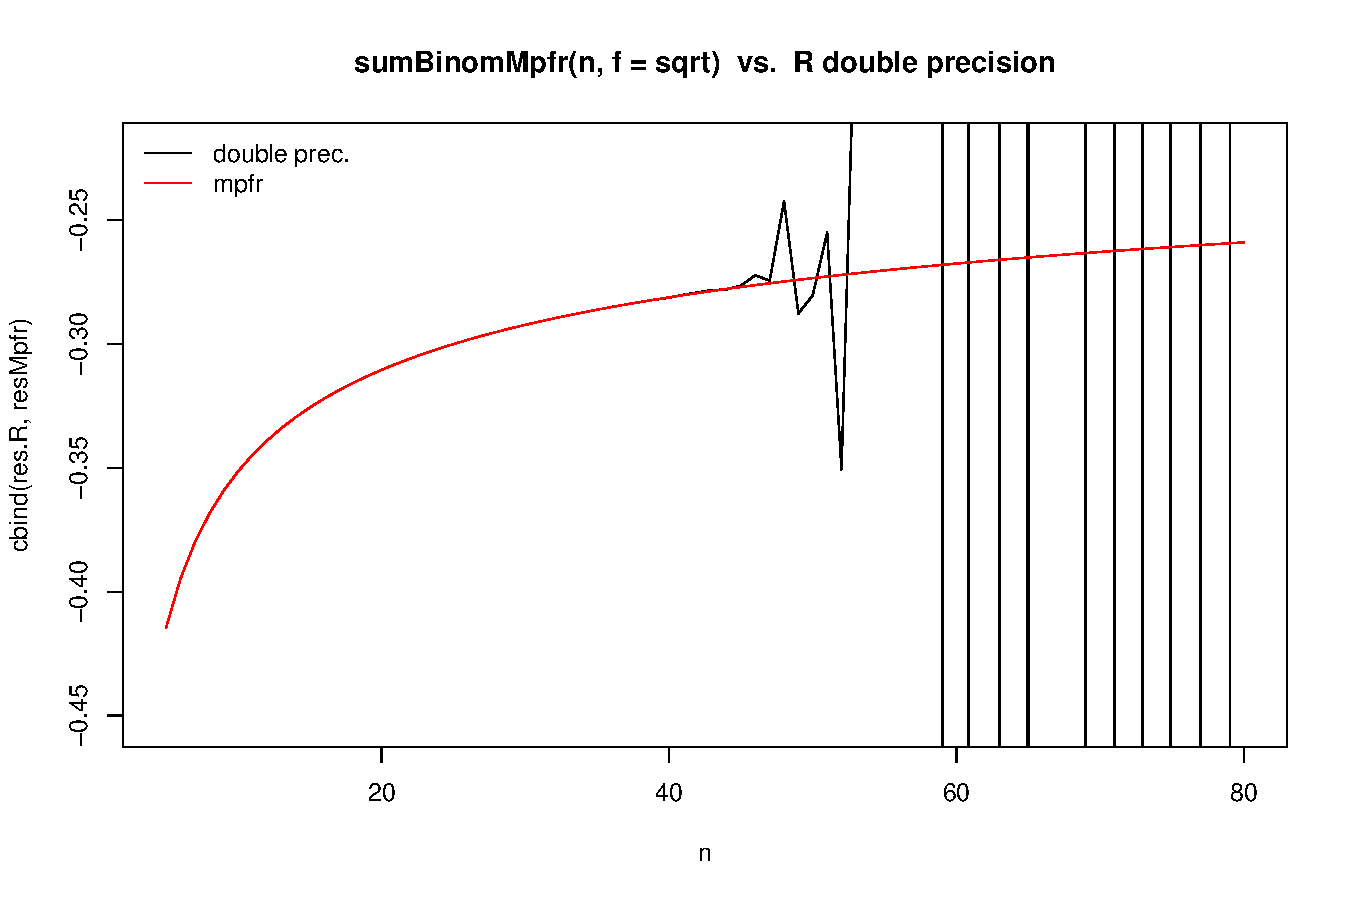
\includegraphics{sumBinC-sqrt-ex-2}
\end{frame}

%%% TeX-master: "Maechler_Rmpfr.tex"

%%     =======
%TODO \input{loglikFrank}
%%     ==========

\section{Capabilities of \pkg{Rmpfr}}


\setkeys{Gin}{width=\textwidth}


\begin{frame}[fragile]\frametitle{Capabilities of \pkg{Rmpfr} -- a Glimpse}
  ``All'' \R arithmetic and math functions just work with ``mpfr''
  numbers:  \\
  Via \code{"Group"} S4 methods

\begin{Schunk}
\begin{Sinput}
> getGroupMembers("Arith")
\end{Sinput}
\begin{Soutput}
[1] "+"   "-"   "*"   "^"   "%%"  "%/%" "/"  
\end{Soutput}
\begin{Sinput}
> getGroupMembers("Compare")
\end{Sinput}
\begin{Soutput}
[1] "==" ">"  "<"  "!=" "<=" ">="
\end{Soutput}
\begin{Sinput}
> getGroupMembers("Math")
\end{Sinput}
\begin{Soutput}
 [1] "abs"      "sign"     "sqrt"     "ceiling"  "floor"    "trunc"   
 [7] "cummax"   "cummin"   "cumprod"  "cumsum"   "exp"      "expm1"   
[13] "log"      "log10"    "log2"     "log1p"    "cos"      "cosh"    
[19] "sin"      "sinh"     "tan"      "tanh"     "acos"     "acosh"   
[25] "asin"     "asinh"    "atan"     "atanh"    "gamma"    "lgamma"  
[31] "digamma"  "trigamma"
\end{Soutput}
\end{Schunk}
\end{frame}

\begin{frame}[fragile]\frametitle{Capabilities of \pkg{Rmpfr} --- 2 ---}
  In addition to the basic arithmetic (including all \code{"Math"} functions!),
  based on the MPFR C library,
  \code{Rmpfr} provides arbitrarily precise versions of

  \begin{itemize}
  \item Bessel functions $j_n(x)$, $y_n(x)$, and $Ai(x)$
  \item Error functions \code{erf(x)}, and \code{erfc(x)}, or equivalently,\\
    \code{pnorm(x)} and \code{pnorm(x, lower.tail=FALSE)}.
  \item Riemann's $\zeta(x) = $\code{zeta(x)},
  \item Exponential integral \code{Ei(x)}
  \item Dilogarithm $\mathrm{Li}_2(x)=$\code{Li2(x)}
  \end{itemize}
\end{frame}

\begin{frame}[fragile]\frametitle{Capabilities of \pkg{Rmpfr} --- 3 ---}
  \begin{itemize}
  \item Arbitarily precise numerical integration (via Romberg), via our
    \code{integrateR()}
    \item Arbitarily root finding (and hence numerical \emph{inverse} function),
      via \code{unirootR()}.
  \end{itemize}
\end{frame}

\begin{frame}[fragile]\frametitle{High precision Matrices}
  Can also do simple arithmetic with \code{"mpfrMatrix"} and
  \code{"mpfrArray"} objects, e.g.
\begin{Schunk}
\begin{Sinput}
> head(x <- mpfr(0:7, 64)/7)
\end{Sinput}
\begin{Soutput}
6 'mpfr' numbers of precision  64   bits 
[1]                       0 0.142857142857142857141 0.285714285714285714282
[4] 0.428571428571428571436 0.571428571428571428564 0.714285714285714285691
\end{Soutput}
\begin{Sinput}
> mx <- x ; dim(mx) <- c(4,2)
> mx[ 1:3, ] + c(1,10,100)
\end{Sinput}
\begin{Soutput}
'mpfrMatrix' of dim(.) =  (3, 2) of precision  64   bits 
     [,1]                   [,2]                  
[1,] 1.00000000000000000000 1.57142857142857142851
[2,] 10.1428571428571428570 10.7142857142857142860
[3,] 100.285714285714285712 100.857142857142857144
\end{Soutput}
\end{Schunk}
\end{frame}

\begin{frame}[fragile]% \frametitle{High precision Matrices}
We can transpose or multiply such matrices, e.g.,
\begin{Schunk}
\begin{Sinput}
> t(mx) %*% 10^(1:4)
\end{Sinput}
\begin{Soutput}
'mpfrMatrix' of dim(.) =  (2, 1) of precision  64   bits 
     [,1]                  
[1,] 4585.71428571428571441
[2,] 10934.2857142857142856
\end{Soutput}
\end{Schunk}
or
\begin{Schunk}
\begin{Sinput}
> crossprod(mx)
\end{Sinput}
\begin{Soutput}
'mpfrMatrix' of dim(.) =  (2, 2) of precision  64   bits 
     [,1]                    [,2]                   
[1,] 0.285714285714285714282 0.775510204081632653086
[2,] 0.775510204081632653086  2.57142857142857142851
\end{Soutput}
\end{Schunk}

\pause
\medskip

and apply works too :
\begin{Schunk}
\begin{Sinput}
> (s7 <- apply(7 * mx, 2, sum))
\end{Sinput}
\begin{Soutput}
2 'mpfr' numbers of precision  64   bits 
[1]  6 22
\end{Soutput}
\end{Schunk}
\smallskip

and, note that \code{all.equal()} methods are provided, as well:
\begin{Schunk}
\begin{Sinput}
> all.equal(s7, c(6,22), tol = 1e-40) # note the tolerance!
\end{Sinput}
\begin{Soutput}
[1] TRUE
\end{Soutput}
\end{Schunk}
\end{frame}

%% ---------------------------------------------------------------------------

\section{Package and Session Information}
\begin{frame}[fragile]%\frametitle{High precision Matrices}
\begin{Schunk}
\begin{Sinput}
> toLatex(sessionInfo())
\end{Sinput}
\begin{itemize}\raggedright
  \item R version 2.14.1 Patched (2012-01-17 r58138), \verb|x86_64-unknown-linux-gnu|
  \item Locale: \verb|LC_CTYPE=de_CH.UTF-8|, \verb|LC_NUMERIC=C|, \verb|LC_TIME=en_US.UTF-8|, \verb|LC_COLLATE=de_CH.UTF-8|, \verb|LC_MONETARY=en_US.UTF-8|, \verb|LC_MESSAGES=de_CH.UTF-8|, \verb|LC_PAPER=C|, \verb|LC_NAME=C|, \verb|LC_ADDRESS=C|, \verb|LC_TELEPHONE=C|, \verb|LC_MEASUREMENT=de_CH.UTF-8|, \verb|LC_IDENTIFICATION=C|
  \item Base packages: base, datasets, graphics, grDevices,
    methods, stats, utils
  \item Other packages: Rmpfr~0.4-5, sfsmisc~1.0-19
  \item Loaded via a namespace (and not attached): gmp~0.5-0,
    tools~2.14.1
\end{itemize}\end{Schunk}
\end{frame}
%%
\begin{frame}[fragile]%\frametitle{....}
\begin{Schunk}
\begin{Sinput}
> packageDescription("Rmpfr")
\end{Sinput}
\begin{Soutput}
Package: Rmpfr
Type: Package
Title: R MPFR - Multiple Precision Floating-Point Reliable
Version: 0.4-5
Date: 2012-01-12
Author: Martin Maechler
Maintainer: Martin Maechler <maechler@stat.math.ethz.ch>
Depends: methods, R (>= 2.11.0)
SystemRequirements: gmp (>= 4.2.3), mpfr (>= 3.0.0)
SystemReqsNotes: MPFR (MP Floating-Point Reliable Library,
       http://mpfr.org/) and GMP (GNU Multiple Precision library,
       http://gmplib.org/), see README
Imports: gmp
Suggests: gmp, polynom
SuggestNotes: 'polynom' is only needed for vignette
URL: http://rmpfr.r-forge.r-project.org/
Description: Rmpfr provides S4 classes and methods for arithmetic
       including transcendental ("special") functions for
       arbitrary precision floating point numbers. To this end, it
       interfaces to the LGPL'ed MPFR (Multiple Precision
       Floating-Point Reliable) Library which itself is based on
       the GMP (GNU Multiple Precision) Library.
License: GPL (>= 2)
Built: R 2.14.1; x86_64-unknown-linux-gnu; 2012-01-19 16:05:40
       UTC; unix

-- File: /tmp/Rmpfr.Rcheck/Rmpfr/Meta/package.rds 
\end{Soutput}
\end{Schunk}
%%---^^^^^^^ or somethings smarter with capture.output() or subsetting ...
my.strsplit(  [["LastChanged"]]  )
\end{frame}


%%% TeX-master: "Maechler_Rmpfr.tex"

% \input{integrateBeta}

\section{Conclusions}
\begin{frame}[fragile]\frametitle{Conclusion}
  \begin{itemize}
  \item  The package \pkg{Rmpfr} allows
 to use arbitrarily high precision numbers
 instead of \R's double precision numbers in many \R\ computations and functions.

\item
 This is achieved by defining S4 classes of such numbers and vectors,
 matrices, and arrays thereof, where all arithmetic and mathematical
 functions work via the (GNU) MPFR C library, where MPFR is acronym for
 ``\emph{\textbf{M}ultiple \textbf{P}recision \textbf{F}loating-Point \textbf{R}eliably}''.
 MPFR is Free Software, available under the LGPL license, and
 itself is built on the free GNU Multiple Precision arithmetic library (GMP).

\item Consequently, by using \pkg{Rmpfr}, you can often call your \R\ function or
 numerical code with mpfr--numbers instead of simple numbers, and all
 results will automatically be much more accurate.

 % Applications by the package author include testing of Bessel or
 % polylog functions and distribution computations, e.g. for stable distributions.
\end{itemize}

\end{frame}

\begin{frame}\frametitle{Executive Summary}
\begin{itemize}%[<+->]
 \item Double precision accuracy (almost 16 digits) is not always sufficient
 \item \pkg{Rmpfr} is here for arbitrarily precise computations in \R.
 \item Many \R functions --- \textbf{when \texttt{source()}d} --- will work
   with ``mpfr''-numbers automagically
   \end{itemize}

\pause

\bigskip

\begin{block}{}
   That's all folks --- with thanks for your attention!
\end{block}
\bigskip

\begin{center}
  Martin M\"achler -- \url{maechler@R-project.org}
\end{center}

\end{frame}

\end{document}

%%% Local Variables:
%%% mode: latex
%%% TeX-command-default: "LaTeX PDF"
%%% TeX-master: t
%%% End:
